% Chapter 3

\chapter{Description of the Setup} % Chapter title
\label{ch:setup} % For referencing the chapter elsewhere, use \autoref{ch:mathtest}

This chapter details the setup that was used in the design of a Swept Source OCT system developed for this thesis work, describing the optical and electrical components that were employed. 

\noindent Particular care will be given to the characterization of the \ac{DAQ} board and the design of the acquisition software. 

\section{Optical Source}
As already discussed in \autoref{ch:theory}, \ac{SS-OCT} systems employ a narrow-bandwidth tunable laser to enable a simple detection scheme and is one of the most critical components of the entire system. The source that was used in this thesis is a SSOCT-1310 by Axsun Technologies, which is a class 3 laser that uses a \ac{MEMS} tunable filter to sweep wavelengths in the 1300 nm range. 

The two most important features of this laser are the fast sweep rate, which enables high speed imaging, and the presence of the $k$-clock signal used for equalizing the nonlinear frequency sweep. 

\begin{figure}[bth]
	\myfloatalign
	{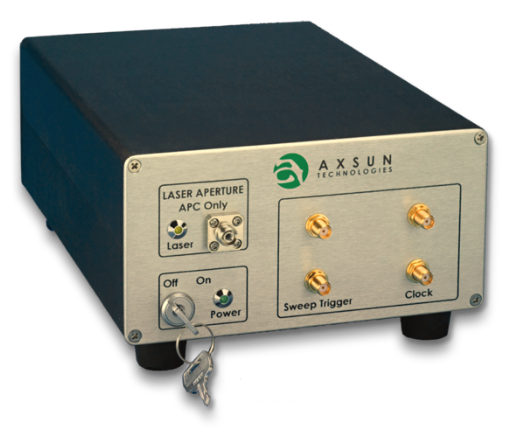
\includegraphics[width=.6\linewidth]{gfx/ch3/axsun}}
	\caption{The acquisition board, AlazarTech ATS9350.}\label{fig:axsun-laser}
\end{figure}

An photo of the laser is available in \autoref{fig:axsun-laser}. The emitted light is collected by connecting a fiber optic patch cord to the FC/APC connector on the front panel, which also includes two SMA connectors for the sweep-start trigger and the $k$-clock signal.


  \begin{table}
	\myfloatalign
	\begin{tabularx}{\textwidth}{Xll} \toprule
		\tableheadline{Parameter} & \tableheadline{Units} & \tableheadline{Value}
		\\ \midrule
		Sweep Rate &  kHz & 100.2 \\
		Center Wavelength & nm & 1305 \\
		Wavelength Tuning Range & nm & 140.38 \\
		Average Power & mW & 25.7 \\
		Duty Cycle & \% & 77.3 \\
		Sampled Duty Cycle & \% & 50.5 \\
		External Clock Min Frequency & MHz & 183.1 \\
		External Clock Average Frequency & MHz & 307.0 \\
		External Clock Max Frequency & MHz & 332.1 \\
		Sampling Clocks & -- & 1536 \\
		\bottomrule
	\end{tabularx}
	\caption{Axsun laser datasheet.}
	\label{tab:axsun-datasheet}
\end{table}

\subsection{Optical Spectrum}
A critical parameter in swept sources for OCT applications is the wavelength interval over which the laser is able to tune. From \autoref{tab:axsun-datasheet}, we can see that the Axsun SSOCT-1310 is centered at $\lambda_0 = 1305$ nm with a bandwidth of $\Delta\lambda = 140.38$ nm. These values were verified by connecting the laser output directly to an \ac{OSA}, measuring its spectrum. 

\begin{figure}[hbt]
	{\myfloatalign
		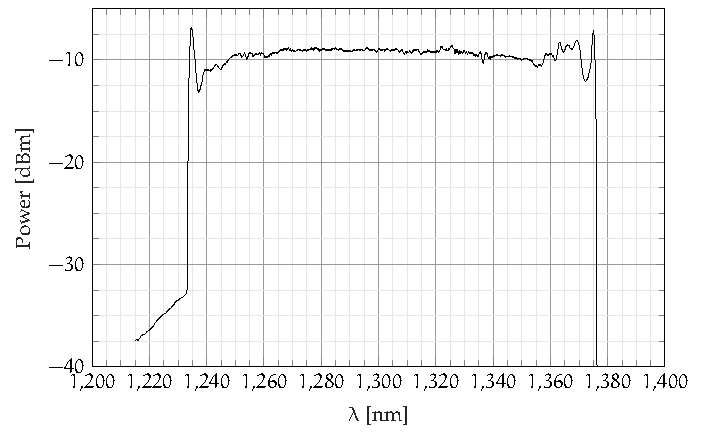
\includegraphics[width=\linewidth]{gfx/tikz/axsun/spectrum}}\\
	\caption{Spectrum of the Axsun SSOCT-1310 laser, obtained with a 1 nm resolution.}\label{fig:axsun-spectrum}
\end{figure}

The measurement was executed with a resolution of 1 nanometer, resulting in the spectrum visible in \autoref{fig:axsun-spectrum}. The edge wavelengths turned out to be $\lambda_1 \approx 1237$ nm and $\lambda_2\approx1376$ nm, which result in a bandwith of $\Delta \lambda \approx 139$ nm and central wavelength of $\lambda_0\approx 1307$ nm. These values slightly differ from those reported in the datasheet, but not enough to compromise the performance of the laser. 

The bandwidth is swept at a frequency $f_a = 100.2$ kHz and with a duty cycle $d_c=0.505$, meaning that the average sweep speed is 
\begin{equation}
\sigma_{\lambda} = \frac{\Delta\lambda f_c}{d_c} \approx 27.8 \,\,\text{nm}/\mu\text{s}.
\end{equation}

Since the goal of SS-OCT sources is to perform a linear frequency sweep, it is more useful to define this parameter in the following manner
\begin{equation}\label{eq:sweep-speed}
\sigma_f = c_0 \left(	\frac{1}{\lambda_0 - \Delta\lambda/2} - \frac{1}{\lambda_0 + \Delta\lambda/2}\right) \frac{f_a}{d_c} \approx 4.9 \,\,\text{THz}/\mu\text{s}
\end{equation}

The istantaneous frequency, after linearization, is thus expressed by 
\begin{equation}
	f(t) = f_0 + \sigma_f t
\end{equation}
where the starting frequency is determined by
\begin{equation}
f_0 = \frac{c_0}{\lambda_0 + \Delta\lambda /2} \approx 218.2 \,\,\text{THz}.
\end{equation}

\subsection{Axial Resolution}
Using \autoref{eq:ss-axial-resolution} and the data provided by \autoref{tab:axsun-datasheet} it is possible to obtain an estimate of the axial resolution provided by the employed optical source. The axial resolution is found to be
\begin{equation}
\delta z \simeq 0.75 \frac{\lambda_0^2}{\Delta \lambda} \approx 9.2 \,\, \mu\text{m.}
\end{equation}

This approximation is valid for sources with a Gaussian spectrum, and can lead to an overestimation of the real axial resolution of the system in case this condition is not met. 

\subsection{Sweep trigger}
The Axsun laser provides a square-wave signal that determines the start of the frequency sweep  and that is used to trigger the acquisition of A-scans. This signal is acquired with a high-speed oscilloscope and illustrated in \autoref{fig:axsun-trigger}. The voltage range was measured as $V_{range} \approx [0 ,1.48] $ V, while the duty cycle is found to be 
\begin{equation}
	d_c = \frac{t_{high}}{t_{high} + t_{low}} \approx 0.97\,.
\end{equation}

For a correct acquisition of A-scans, the datasheet recommends to trigger the acquisition device when the signal level reaches the value of $V_{trig} = 0.71$ V, pictured in \autoref{fig:axsun-trigger} with a red line. 


\begin{figure}[hbt]
	\myfloatalign
	{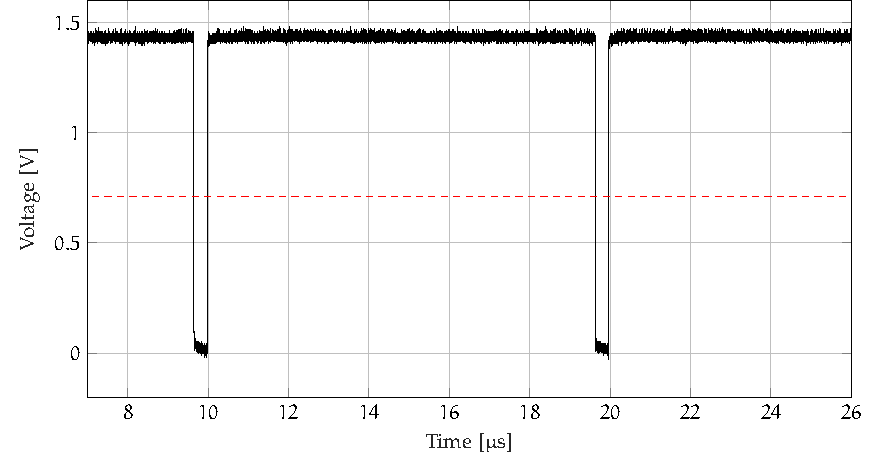
\includegraphics[width=0.8\linewidth]{gfx/ch3/trigger}}\\
	\caption{Sweep trigger of the SSOCT-1310 laser.}\label{fig:axsun-trigger}
\end{figure}

\subsection{Power profile}
Using a photodiode it's possible to measure the istantaneous power profile of the laser emission. The photodiode generates an electrical current which is proportional to the power of the detected electromagnetic field: 
\begin{equation}
	I_{ph} = \mathcal{R} \cdot P 
\end{equation}
The constant $\mathcal{R}$ is called \emph{responsivity} [A/W] and is specific to the detector used. The current can then be measured with an oscilloscope. In order to avoid the saturation of the receiver, a 3 dB coupler was inserted between the source and the photodiode. The obtained power profile is depicted in \autoref{fig:axsun-power} along with the sweep trigger. We can observe that in the first $\sim 5$ $\mu$s after the positive edge of the trigger, the istantaneous power behaves like a typical laser pulse while outside of this interval it assumes an irregular profile. 


\begin{figure}[hbt]
	\myfloatalign
	{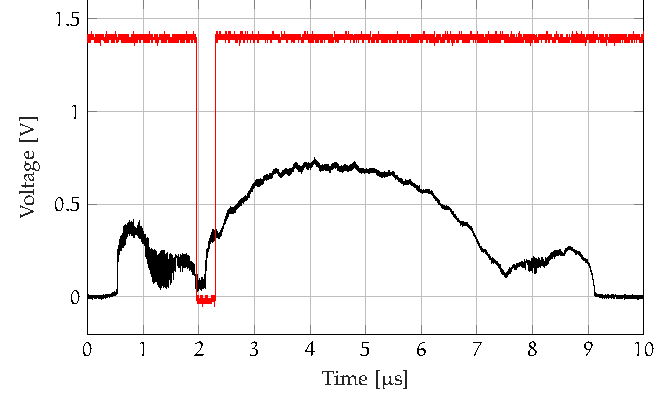
\includegraphics[width=0.8\linewidth]{gfx/ch3/power-profile}}\\
	\caption{Sweep trigger of the SSOCT-1310 laser.}\label{fig:axsun-power}
\end{figure}


\subsection{k-clock}
As already stated, this particular SS-OCT laser is equipped with an internal \ac{MZI} which generates the variable-frequency clock, called $k$-clock, used to sample the A-scan signal at a variable rate and equalize the nonlinear terms in the frequency sweep. As we can see in \autoref{fig:kclock}, this signal assumes values in the $[0, 900]$ mV range with an average value of about 460 mV. This sinusoidal signal will be used to drive the acquisition board for the first $5$ $\mu$seconds of the sweep and from this point forward will be referred to as \emph{useful clock}. As per \autoref{tab:axsun-datasheet}, the total number of samples that cab be acquired using this clock is $N_s = 1536$. In the last 5 $\mu$seconds the clock is called "dummy" because of its undefined behaviour that could lead to issues in the clocking of the DAQ devices.

\begin{figure}[hbt]
	\myfloatalign
	{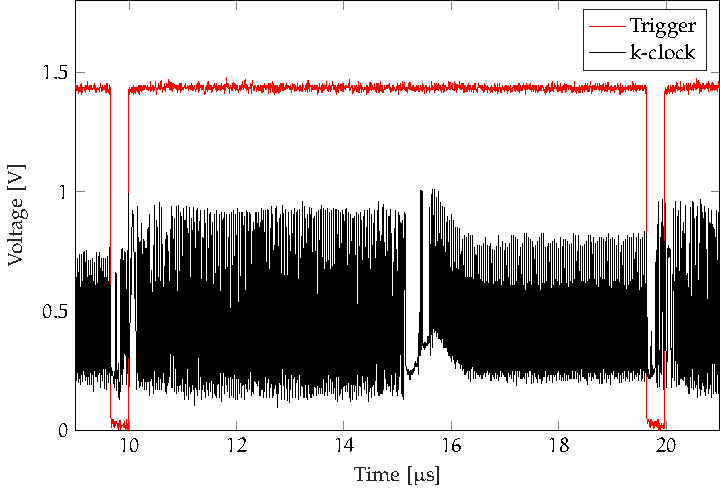
\includegraphics[width=0.8\linewidth]{gfx/ch3/clock}}\\
	\caption{Estimate of the istantaneous frequency of the k-clock.}\label{fig:kclock}
\end{figure}

In \autoref{fig:clock-zoom} are depicted two 50 nanoseconds windows at the start (left) and in the middle (right) of the useful clock, where the variable frequency of signal is clearly visible. Also worth noting is that at the start of the sweep the signal appears much more distorted than in the middle of the sweep. Fortunately, this behaviour did not compromise the performance of the system. 

\begin{figure}[bth]
	\myfloatalign
	{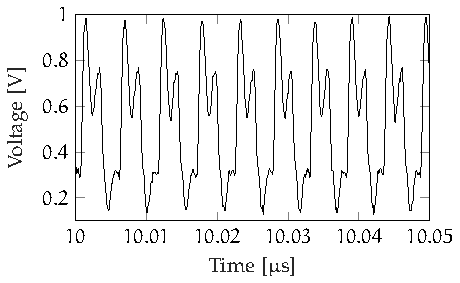
\includegraphics[width=.45\linewidth]{gfx/ch3/clock1}} \quad
	{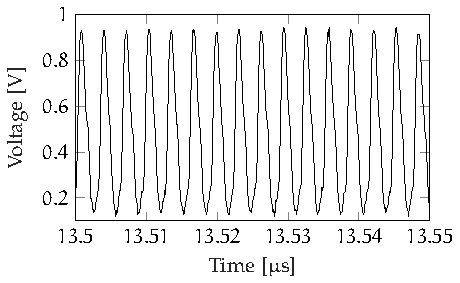
\includegraphics[width=.45\linewidth]{gfx/ch3/clock2}} \\
	\caption{Behaviour of the useful k-clock at different time instants.}\label{fig:clock-zoom}
\end{figure}

To gain further insights on the nature of the frequency sweep, it is interesting to estimate the istantaneous frequency of the k-clock. A method to perform this estimate is the following
\begin{enumerate}
	\item Subtract the average value from the signal
	\item Interpolate the signal $(t, y)$ to obtain $(\hat{t}, \hat{y})$
	\item Determine the time instants $\hat{t}_i$ at which the signal $\hat{y}$ crosses 0, from which a vector $\mathcal{I} = \left[\hat{t}_{i_1}, \hat{t}_{i_2}, \dots,  \hat{t}_{i_N}\right]$ is built.
	\item Compute the difference between the adjacent elements of $\mathcal{I}$ and obtain $\mathcal{T} = \left[\hat{\tau}_{i_1}, \hat{\tau}_{i_2}, \dots,  \hat{\tau}_{i_{N-1}}\right]$,
	\item The istantaneous frequency of the signal is then estimated as $\hat{f}_i = 1/2 \hat{\tau}_i$.
\end{enumerate} 

The result of this method is illustrated in \autoref{fig:kclock-frequency}. Since the estimate is rather noisy, a low pass filter was applied to the $\hat{f}_i$ signal, resulting in a much cleaner estimation (depicted in red). As we can observe, the istantaneous frequency rapidly changes at the start and at the end of the sweep, while in the middle it stabilizes at about 320 MHz. Since a constant k-clock frequency implies a linear frequency sweep, we can infer that the sweep nonlinearities are much more prevalent at the edge of the sampling interval. 

The maximum estimated frequency is $\hat{f}_{clk}^{max} = 339$ MHz, as opposed to the value that was reported in \autoref{tab:axsun-datasheet} of $f_{clk}^{max} = 332.2$ MHz. This slight overestimation is also visible in \autoref{fig:kclock-frequency}, where we can see that the low-pass filtered signal is slightly higher than the average value of the non filtered one.

\begin{figure}[hbt]
	\myfloatalign
	{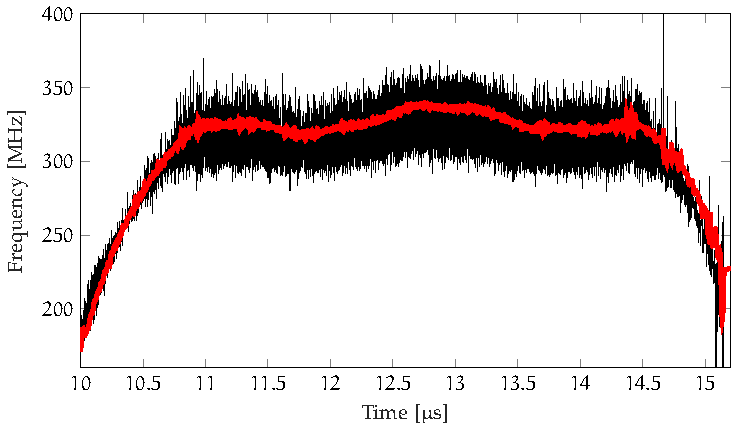
\includegraphics[width=0.8\linewidth]{gfx/ch3/lowpass}}\\
	\caption{Estimate of the istantaneous frequency of the k-clock.}\label{fig:kclock-frequency}
\end{figure}

From the maximum frequency of the k-clock signal we can measure the maximum imaging depth obtainable by the system. 

Two replicas of the pulse overlapping with a relative time delay $\tau$ will generate a beat frequency $f_b$ given by

	\begin{equation}
		f_b = \sigma_f \tau
	\end{equation}
	
where $\sigma_f$, the sweep speed, was determined in \autoref{eq:sweep-speed}. In a OCT setup, the time delay $\tau$ is related to the path mismatch of reference and sample arm, which in turn depends on the depth of the layer of the sample that generates the reflection. In this way	
	\begin{equation}
		\tau = \frac{2dn}{c_0},
	\end{equation}
where $c_0$ is the speed of light in vacuum, $n$ is the refractive index of the sample and $d$ is the depth. By the Nyquist theorem, the maximum beat frequency that can be digitized using the $k$-clock is
	
	\begin{equation}
		f_b^{max} = \frac{f_{clk}^{max}}{2},
	\end{equation}
which results in a maximum depth in air ($n=1$) of  
	\begin{equation}
		d_{max} = \frac{c_0 f_{b}^{max}}{2\sigma_f}  =  \frac{c_0 f_{clk}^{max}}{4\sigma_f} \simeq 5.1 \text{ mm}.
	\end{equation}

\subsection{Coherence length}
In \autoref{ch:theory} we have seen that the coherence length of a source is one of the most important parameters of optical sources, independently of the type of OCT system. In \ac{TD-OCT}, this parameter determines the axial resolution of the system, while \ac{FD-OCT} schemes it also affects the imaging range, as the reference arm is fixed. In particular, complex conjugate artifacts arising from the Fourier trasform of the detected signals halve the maximum imaging range. For this reason, the coherence length of a swept source satisfies the following inequality
\begin{equation}
	l_c \geq 2 \cdot d_{max},
\end{equation}
which implies that the coherence length of the SSOCT-1310 source is at least
\begin{equation}
	l_c \geq 2\cdot d_{max} \approx 10.2 \text{ mm.}
\end{equation}

The exact value was experimentally determined in \cite{Calabrese2017}, measuring the normalized coherence function $|\gamma(\Delta z)|$ by placing a mirror in the sample arm and acquiring the interference signal for different values of \ac{OPD}. The path length difference was changed by translating the reference mirror. The intensity of the interference signal, normalized by its maximum value, is plotted in  \autoref{fig:axsun-coherence-length} as a function of the \ac{OPD}. When the \ac{OPD} increases above a certain value, the coherence function decays exponentially as
\begin{equation}
|\gamma(\Delta z)| \propto e^{-\alpha |\Delta z|},
\end{equation}
which corresponds to a linear decay in the logarithmic domain. The parameter $\alpha$ was estimated by fitting the data points to a line using a Least-Squares fit. The coherence length is finally determined as the $\Delta z$ value such that $|\gamma(\Delta z)| = 1/2$, resulting in
\begin{equation}
	l_c = 2 \cdot \frac{\ln 2}{\alpha} \approx 12.3 \text{ mm.}
\end{equation}


\begin{figure}[hbt]
	\myfloatalign
	{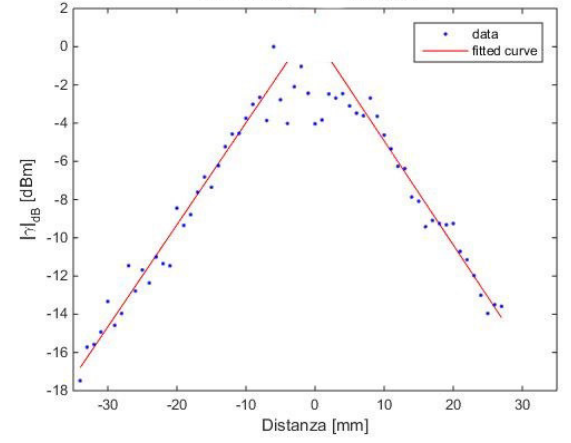
\includegraphics[width=0.8\linewidth]{gfx/ch3/axsun-coherence-length}}\\
	\caption{Experimental estimation of the normalized coherence function.}\label{fig:axsun-coherence-length}
\end{figure}

\newpage

\section{Scanning System}
One of the most critical components of an OCT is the scanning system. Its role is to receive the light emitted by the source, focus it on the sample under test, and collect the backreflections. A scanning system usually comprises of three different devices

\begin{enumerate}
	\item Fiber collimator
	\item Galvanometric Mirrors
	\item Focusing lens
\end{enumerate}

\begin{figure}[bth]
	\myfloatalign
	{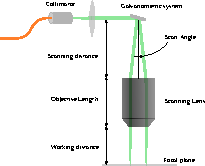
\includegraphics[width=0.8\linewidth]{gfx/setup-diagrams/scanning-diagram.pdf}}
	\caption{Diagram of a OCT scanning system.}\label{fig:scanning-diagram}
\end{figure}

A schematic of this system is depicted in \autoref{fig:scanning-diagram}. Light coming from a single mode optical fiber is deflected by a system of galvanometric mirrors towards a lens which in turns focuses the radiation on the sample. By rotating the mirrors the light beam is focused on a different position on the sample. The reflected beam travels the same path in the opposite direction and is collected by the optical fiber. The correct design of these components is paramount in order to guarantee small transversal and axial resolutions of the OCT system. 



\subsection{Collimator}
The role of the fiber collimator is to collect light coming from a single mode fiber and collimate the beam on the galvanometric mirrors. The divergence angle at the output of the collimator is approximated with the following equation when the beams have a Gaussian intensity profile:
\begin{equation}
	\theta \approx \frac{D}{f} \frac{180}{\pi},
\end{equation}
where $D$ is the mode diameter and $f$ is the focal length of the collimator. This approximation works well for sigle mode fibers, but will underestimate the real divergence angle in the case of multimode fibers, as the intensity profile has a non-Gaussian shape. 

The collimator used in this setup is the Thorlabs F280APC-C\footnote{\url{https://www.thorlabs.com/thorproduct.cfm?partnumber=F280APC-C}}, which is designed to work in the 1310 nm range. Its main specifications are summarized in \autoref{tab:collimator-datasheet}. 

\begin{table}[h]
	\myfloatalign
	\begin{tabularx}{\textwidth}{Xll} \toprule
		\tableheadline{Parameter} & \tableheadline{Units} & \tableheadline{Value}
		\\ \midrule
		Central wavelength & nm & 1310 \\
		Beam diameter & mm & 3.4 \\
		Divergence angle & degrees & 0.028 \\
		Lens numerical aperture (NA) & -- & 0.15 \\
		Focal length & mm & 18.67 \\
		\bottomrule
	\end{tabularx}
	\caption{Thorlabs F280APC-C datasheet.}
	\label{tab:collimator-datasheet}
\end{table}

\subsection{Scanning lens}
The light beam deviated by the galvanometric mirrors has to be focused on the sample under test in order to guarantee high resolution images. This is accomplished by a telecentric focusing lens. This type of lenses is characterized by flat image planes which are ideal for OCT applications. 

The main parameters that characterize this device are the following:
\begin{itemize}
	\item Entrance Pupil Size (EP): it specifies the diameter of the collimated laser beam that will maximize the resolution of the imaging system. When using a single galvanometric mirror, the EP is located at the pivot point of the mirror. When two mirrors are used, the EP is located between the two mirrors. 

	\item Scanning Distance (SD): the distance between the EP and the base of the lens. 
	
	\item Scan Angle (SA): the angle between the incoming light beam and the optical axis of the lens. 
	
	\item Working Distance (WD): the distance between the tip of the lens and the focal plane.
	
	\item Parfocal Distance (PD): the distance between the base of the lens and the focal plane. It is equal to the WD plus the objective length.
	
	\item Field of View (FOV): the area on the focal plane that can be imaged with a resolution equal or better than the one guaranteed by the lens. 
	
	\item Depth of View (DOV): it corresponds to the distance between parallel planes on either side of the focal plane, where the beam spot diameter is $\sqrt{2}$ greater than it is at the focal plane. Using lenses with a high DOV value yields images with high lateral resolution in a larger interval of depths. 
	
	\item Spot size: the diameter of the beam on the focal plane. 
\end{itemize}


 The lens used for the SS-OCT system developed in this thesis is the Thorlabs LSM04\footnote{\url{https://www.thorlabs.com/thorproduct.cfm?partnumber=LSM04}}. Its main specifications are listed in \autoref{tab:lens-datasheet}. A simulation of the beam spot size on the focal plane is available in \autoref{fig:spotsize}, where we can see that it increases for bigger scan angles. This behaviour has the effect of reducing the lateral resolution at the edge of the FOV. 
 
\begin{figure}[bth]
 	\myfloatalign
 	{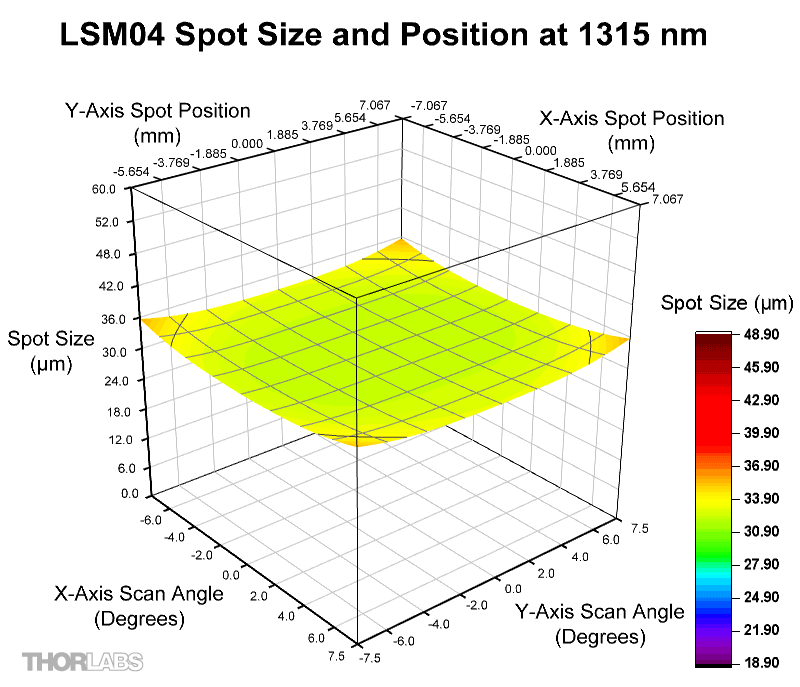
\includegraphics[width=0.6\linewidth]{gfx/ch3/spotsize}}
 	\caption{The Thorlabs GVS002 galvo system.}\label{fig:spotsize}
 \end{figure}
 
 
 
 \begin{table}[h]
 	\myfloatalign
 	\begin{tabularx}{\textwidth}{Xll} \toprule
 		\tableheadline{Parameter} & \tableheadline{Units} & \tableheadline{Value}
 		\\ \midrule
 		Wavelength range & nm & 1250-1380\\
 		Effective Focal Length (EFL) & mm & 54 \\
 		Entrance Pupil size & mm & 4 \\
 		Working Distance & mm & 42.3 \\		
 		Parfocal Distance & mm & 80.8 \\
 		Scan Distance & mm & 18.9 \\
 		Maximum Scan Angle & degrees & $\pm 7.5 \times \pm 7.5$ \\
 		Field of View & mm$^2$ & $14.1 \times 14.1$ \\
 		Depth of View & mm & 0.61\\
 		\bottomrule
 	\end{tabularx}
 	\caption{Thorlabs LSM04 datasheet.}
 	\label{tab:lens-datasheet}
 \end{table}
 
 
 
 \subsubsection{Lateral resolution}
 
 Using the parameters listed in \autoref{tab:lens-datasheet} it is also possible to obtain an estimate of the lateral resolution of the system, which is dictated by the diffraction limited spot size of the focused optical beam. For Gaussian-shaped beams, it is approximated as \cite{Drexler2015}
 \begin{equation}
 	\delta x \simeq \frac{4\lambda_0}{\pi} \frac{f}{d}
 \end{equation}
 where $\lambda_0$ is the central wavelength of operation, $f$ is the focal length of the lens and $d$ is the diameter of the beam at the entrance of the lens. The lateral resolution guaranteed by the LSM04 is thus
 \begin{equation}
 	\delta x \simeq \frac{4\lambda_0}{\pi} \frac{EFL}{EP} \approx 22.5 \,\,\mu\text{m.}
 \end{equation}
 
 Since the diameter of the beam exiting the fiber collimator is slightly smaller ($d=3.4$ mm) than the EP size, the resulting lateral resolution becomes
 \begin{equation}
	\delta x \approx 26.5 \,\,\mu\text{m}.
 \end{equation}
 
 The depth of view, also called confocal parameter, limits the imaging depth of the system. Due to diffraction, this paramer is also governed by the lateral resolution of the system through the following equation
 \begin{equation}
	 b = \frac{2 \delta x^2}{\lambda_0}.
 \end{equation}
 
 This effect is illustrated in \autoref{fig:na}, where we can see that using lenses with a high numerical aperture (NA), or small spot size, the depth of view is limited. In OCT systems it is preferred to use low NA lenses to sacrifice lateral resolution in favor of a depth of view comparable to the coherence length of the source. Following this criterion the coherence length is fully exploited. 
 
  \begin{figure}[bth]
 	\myfloatalign
 	{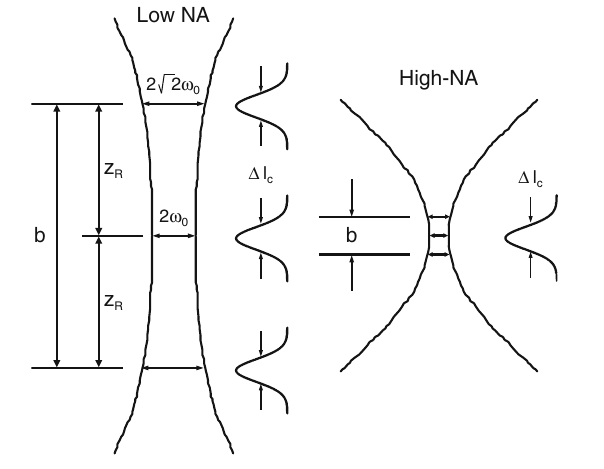
\includegraphics[width=0.6\linewidth]{gfx/ch3/na}}
 	\caption{Basic diagram of a  SS-OCT setup}\label{fig:na}
 \end{figure}
 
 
 Using the EP size when calculating $\delta x$, the confocal parameter is $b \approx 0.61$ mm, equal to the value reported in \autoref{tab:lens-datasheet}, while using the beam size diameter $d = 3.4$ mm it becomes $b \approx 0.84$ mm. 
 
 

\subsection{Galvanometric Mirrors}

In order to acquire B-scans and C-scans it is necessary to direct the laser beam emitted from the swept laser over a speficied area of the sample. This is accomplished by using a system of \emph{galvanometric mirrors}, also called \emph{galvo mirrors}. A cross-sectional image can be generated with a single 1D mirror, that is, a mirror which can rotate on a single axis, while volumetric data require the use of either a 2D mirror or a couple of 1D mirrors. In the second case, each mirror is responsible for the movement of the beam over a single direction on the focal plane, typically called X and Y. 

\begin{figure}[bth]
	\myfloatalign
	{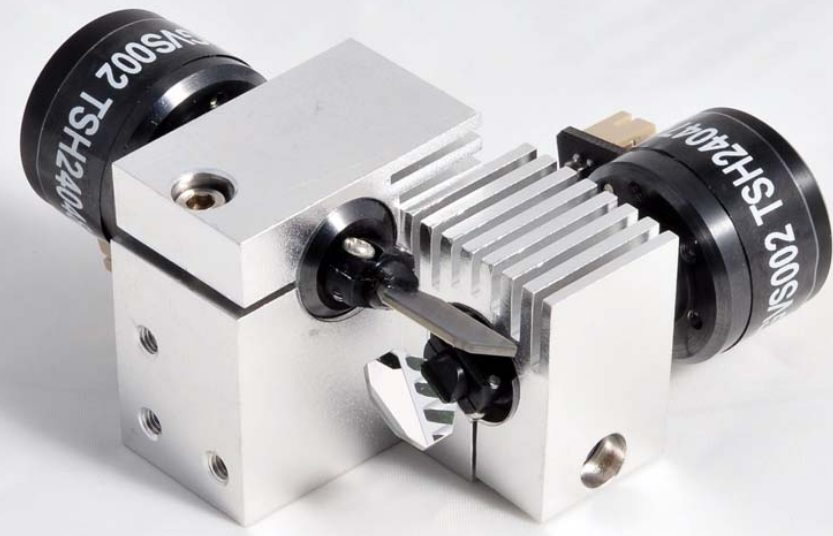
\includegraphics[width=0.6\linewidth]{gfx/ch3/galvo}}
	\caption{The Thorlabs GVS002 galvo system.}\label{fig:galvo}
\end{figure}

The galvo system employed in this thesis work is the Thorlabs GVS002\footnote{\url{https://www.thorlabs.com/thorproduct.cfm?partnumber=GVS002}}, which consists in two 1D silver plated mirrors, the motors that controls them, a detector to measure the mirrors' position  and the servo driver boards that interpret the error signals coming from the detector to correctly drive the motors to the demanded position. A photo of the dual axis motor/mirror assembly is available in \autoref{fig:galvo}. A thorough analysis of the electrical circuitry of the system and its performance characterization is found in \cite{Calabrese2017}. 

\subsubsection{Controlling the mirrors}
The position of each mirror is controlled by sending a voltage signal to the respective driver board which is proportional to the mechanical angle of the respective motor. The maximum mechanical scan angle that the GVS002 system can handle is $\pm 12.5^\circ$, but it can vary depending on the laser beam diameter and the voltage scaling factor. This particular galvo system offers three different scaling factors which also govern the maximum input voltage applied to the servo boards:

\begin{center}
\begin{tabularx}{\textwidth}{lll} \toprule
	\tableheadline{Scaling factor} & \tableheadline{Max. voltage} & \tableheadline{Max. scan angle}
	\\ \midrule
	0.5 V/$^\circ$ & $\pm 6.25$ V & $\pm 12.5^\circ$ \\
	0.8 V/$^\circ$ & $\pm 10$ V & $\pm 12.5^\circ$ \\
	1 V/$^\circ$   & $\pm 10$ V & $\pm 10^\circ$ \\
	\bottomrule
\end{tabularx}
\end{center}




Through simple trigonometric, it can be shown that the scan angle seen by the focusing lens, called \emph{optical scan angle}, $\theta_o$, is twice the mechanical scan angle applied to the mirror, $\theta_m$. Setting the scaling factor  $\alpha = 1 V/^\circ$, the maximum optical scan angle then becomes $\pm 20^\circ$, which allows us fully exploit the maximum angle supported by the lens. In this case, the full FOV is scanned if the applied voltage is $v_{max} = \pm 7.5^\circ/(2\alpha) = \pm 3.75$ V. 

The beam spot position on the focal plane is related to the mechanical angle applied to the mirrors and the focal length of the lens through the following relation

\begin{align}
	x = EFL \tan(2 \theta_{m,x})\label{eq:focusplane-positionx}\\
	y = EFL \tan(2 \theta_{m,y})\label{eq:focusplane-positiony}
\end{align}

With a scaling factor equal to $\alpha$, the voltage signal $v_{x,y}(t)$ will therefore focus the beam at the following position
\begin{align}
x(t) = EFL \tan\left[2 \alpha v_x(t) \frac{\pi}{180}\right]\\
y(t) = EFL \tan\left[2 \alpha v_y(t) \frac{\pi}{180}\right]
\end{align}

The two signals $v_x$ and $v_y$ are delivered to the driver boards as two pairs of positive voltage signals, $(v_x^+, v_x^-)$ and $(v_y^+, v_y^-)$, where

\begin{equation}
	v_i^+(t) = \begin{cases}
		v_i(t) & v_i(t) \geq 0\\
		0 & v_i(t) < 0
 	\end{cases},
 	 	\quad v_i^-(t)=
 	\begin{cases}
		-v_i(t) & v_i(t) < 0\\
		 0 & v_i(t) \geq 0
 	\end{cases}
\end{equation}


\subsubsection{Image distortion}
When using a two-mirror system three different effects can appear
\begin{enumerate}
	\item The arrangement of the mirrors leads to a distortion of the image field, which will be "pillow-shaped" instead of rectangular (fig:galvo-distortion). This is due to the fact that the distance between the two mirrors depends on the mechanical angle applied to the mirrors. 
	
	
	\begin{figure}[bth]
		\myfloatalign
		{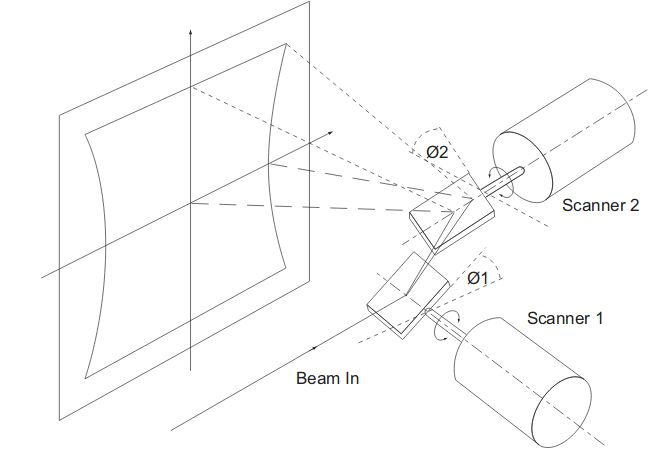
\includegraphics[width=0.75\linewidth]{gfx/ch3/galvo-distortion}}
		\caption{Field distortion using two mirrors.}\label{fig:galvo-distortion}
	\end{figure}
	
	
	\item From \autoref{eq:focusplane-positionx} and \autoref{eq:focusplane-positiony} we can notice that the distance on the image field is not directly proportional to the applied angle but to its tangent. This can result in an additional distortion effect. 
	
	\item If an ordinary lens is used for focusing the laser beam, the focus lies on a sphere.
	In a flat image field, a varying spot size results. 
\end{enumerate}


\begin{figure}[bth]
	\myfloatalign
	{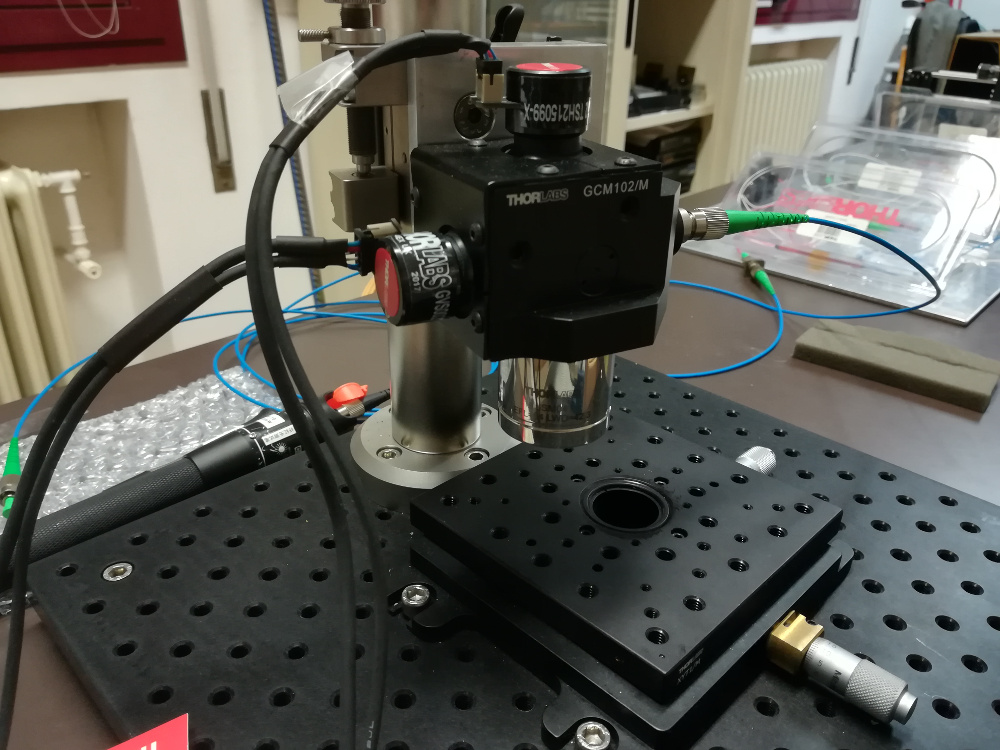
\includegraphics[width=0.75\linewidth]{gfx/ch3/testa}}
	\caption{The final scanning system mounted on a movable vertical support.}\label{fig:testa}
\end{figure}
	
	\newpage
\section{Acquisition Board}
	
	In order to digitize the interference signals generated by the OCT system and reconstruct images of the analyzed sample in real time, a specialized high speed \acf{DAQ} device is required. A desired feature in a \ac{DAQ} board for SS-OCT applications is the ability to sample the signals at a variable rate using a supplied $k$-clock, avoiding the computationally heavy task of data resampling and allowing higher imaging speeds. The \ac{DAQ} board used for this thesis is the AlazarTech ATS9350\footnote{\url{http://www.alazartech.com/product/ats9350}}, which is a specialized digitizer ideal for OCT, ultrasonic and radar applications. 
	
	
	\begin{figure}[bth]
		\myfloatalign
		{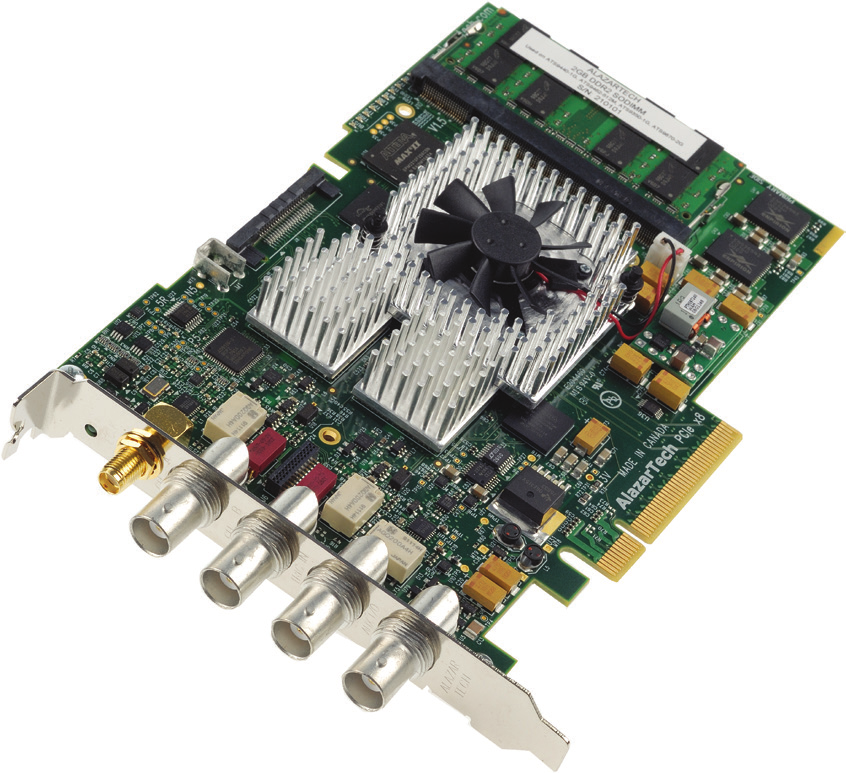
\includegraphics[width=.6\linewidth]{gfx/board}}
		\caption{The acquisition board, AlazarTech ATS9350.}\label{fig:acq-board}
	\end{figure}

	This device is an 8-lane PCI Express 2.0 (PCIe x8) card with the following characteristics:
	\begin{itemize}
		\item 12 bits sample resolution
		\item 250 MHz input bandwidth
		\item 2 input channels with a dedicated \ac{ADC} chip and a user selectable sampling rate which ranges from 2 MHz up to 500 MHz. The raw throughput to the on-board memory is thus $T = 2 \text{ bytes per sample} \times 2 \text{ channels} \times 500 \text{MHz} = 2 \text{ GB/s}$.
		\item User selectable input voltage range, from $\pm 40$ mV to $\pm 4$ V for a better utilization of the 12 bit resolution.
		
		\item External trigger support
		\item Variable frequency external clocking
		\item AUX (Auxiliary) connector that can be configured either as a trigger output or a "acquisition start" trigger. 
		
		\item dual-port 128 Megasamples on-board memory
		
		\item On board \ac{FPGA} module for the computation of the \ac{FFT} on one of the input channels. 
		
	\end{itemize}


	The board also comes with the proprietary AlazarDSO software to configure the device, acquire and display signals. For custom applications, the board can be integrated using a supplied \ac{SDK} which includes libraries and headers for a variety of different programming languages, including C/C++, Python and MATLAB. The device was installed in a Dell Precision T5810\footnote{\url{https://www.dell.com/us/business/p/precision-t5810-workstation/fs}} workstation with the following specifications:
	\begin{itemize}
		\item Intel Xeon E5-1650 v4, 3.6 GHz, 6 cores, 12 threads
		\item 16 GB of DDR4 ECC RAM at 2400 MHz
		\item 256GB SATA SSD
		\item NVIDIA Quadro M4000 with 8 GB of DDR5 memory
	\end{itemize}
	

    \subsection{Data Acquisition}
    
    Data acquisition on the ATS9350 is organized in \emph{records} and \emph{buffers}. A record consists in a user defined number of samples acquired by the board for each trigger event. In OCT applications, a record typically corresponds to a single A-scan. A buffer instead is a collection of records and is the format in which data is returned to the user application. For our application, a buffer corresponds to a B-scan. 
    
    This \ac{DAQ} board can be configured to acquire data in one of the following modes
    \begin{enumerate}
    	\item Single-Port mode acquires data to the on-board memory and then, after the acquisition is complete, transfers data to the host PC memory. This mode can be used if the application can tolerate to miss trigger events that occur while data is being transferred. 
    	
    	\item Dual-Port mode, also called AutoDMA, acquires to on-board memory while, at the same time, trasferring data from on-board memory to the host PC memory. This is the preferred acquisition method, as no trigger events are missed by the board while managing the data transfer, meaning that no B-scans are lost by the system. The on-board memory acts as a very long \ac{FIFO} structure that is able to stream data to the host memory at the rate supported by the motherboard. 
    	
    	The benchmarking tool integrated in the AlazarDSO software measured an average PCIe throughput of $1.735$ GB/s, which is even higher than that advertised by AlazarTech. 
   	
    	    	
    \end{enumerate}


\begin{figure}[bth]
	\myfloatalign
	\subfloat[Acquisition using Single-Port Memory.]
	{\label{fig:single-port-acq}
		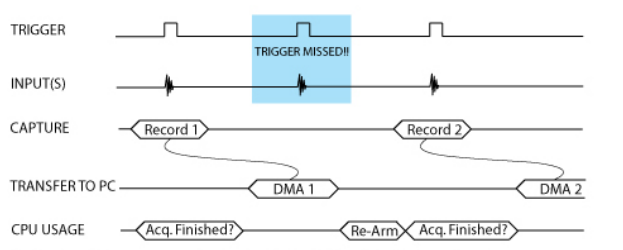
\includegraphics[width=.75\linewidth]{gfx/single-port-acq}} \\
	\subfloat[Acquisition using Dual-Port Memory.]
	{\label{fig:dual-port-acq}
		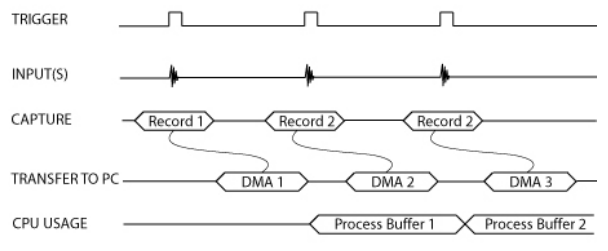
\includegraphics[width=.75\linewidth]{gfx/dual-port-acq}}
	\caption{Diagram highlighting the differences between Sigle-Port acqusitions and Dual-Port acqusitions}\label{fig:single-vs-dual-port}
\end{figure}
    
    In \autoref{fig:single-vs-dual-port} a comparison between the two acquisition techniques is available. For single-port acquisitions, in \autoref{fig:single-port-acq} we can see that trigger events happening while the \ac{DMA} transfer is ongoing are missed completely, and virtually all CPU cycles are used in managing the data acquisition. This leaves no room for data processing on the CPU. In Dual-port AutoDMA acquisition instead (\autoref{fig:dual-port-acq}) no trigger events are missed and over 95\% of CPU time is available for data processing. 
    
    This is possible thanks to proprietary circuitry that allows for data transfers to be initiated by the hardware itself, without the need to waste CPU cycles. On the software side, an asynchronous driver is able to parallelize the tasks of setting up a DMA channel while handling data transmission on another channel. 


	The board supports diffent types of AutoDMA acquisitions which will be here shortly explained 

	\subsubsection{Traditional AutoDMA}
	This method allows for the acquisition of both pre-trigger and post-trigger data, which will be returned to the user is form of buffers that contain from 1 to 8192 records, one for each trigger event. Each record can come with its own header containing a 40-bit timestamp. A DMA transfer is initiated after the acquisition of each record, copying the data from on-board to user supplied memory.
	
	 \begin{figure}[bth]
		\myfloatalign
		{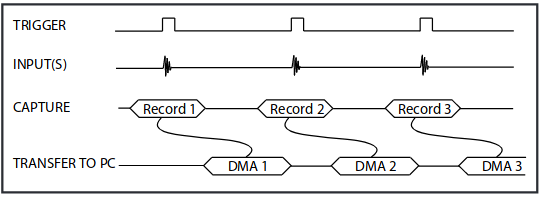
\includegraphics[width=.75\linewidth]{gfx/ch3/traditional-autodma}}
		\caption{Time diagram of a Traditional AutoDMA acquisition.}\label{fig:traditional-autodma}
	\end{figure}
	
	Fast trigger repeat rates are not supported and can cause the board to overflow even if data transfer is happening at the maximum sustained rate and the on-board memory has not been completely used up. 
	
	\subsubsection{NPT AutoDMA}
	No Pre-Trigger (NPT) AutoDMA is designed for applications that do not require the acquisition of data before a trigger event. By only storing post-trigger data, the memory bandwidth is optimized. Record headers are also not included, resulting in a more efficient memory utilization. For this reason NPT AutoDMA supports high trigger repeat rates resulting in an acquisition speed which is only limited by the PCIe transfer speed and the rate at which the user application consumes data. 
	
	\begin{figure}[bth]
		\myfloatalign
		{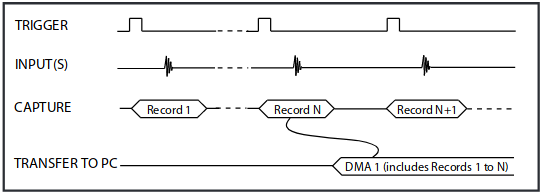
\includegraphics[width=.75\linewidth]{gfx/ch3/npt-autodma}}
		\caption{Time diagram of a NPT AutoDMA acquisition.}\label{fig:npt-autodma}
	\end{figure}

	Unlike Traditional AutoDMA, a DMA transfer is initiated only after an entire buffer consisting of multiple records is acquired. This data acquisition method has been specifically designed for ultrasonic scanning, radar and medical imaging applications such as OCT. 
    
    \subsection{FFT module}
    The ATS9350 is equipped with a \ac{FPGA} module that computes the FFT on data records acquired on the first of the two input channels. For OCT applications this means that a powerful GPU dedicated to data processing is not needed, simplyfing the user application both on the design and efficiency standpoint. In \autoref{fig:fft-module} the flow diagram of the FFT module is available: a data record is zero-padded to a power-of-2 length (and a maximum of 2048), multiplied by a complex windowing function and fed to the FFT module, whose output is then scaled and optionally converted in a logarithmic scale. At the end of the chain it is possible to obtain either FFT data, time-domain data or both. 
    
    \begin{figure}[bth]
    	\myfloatalign
    	{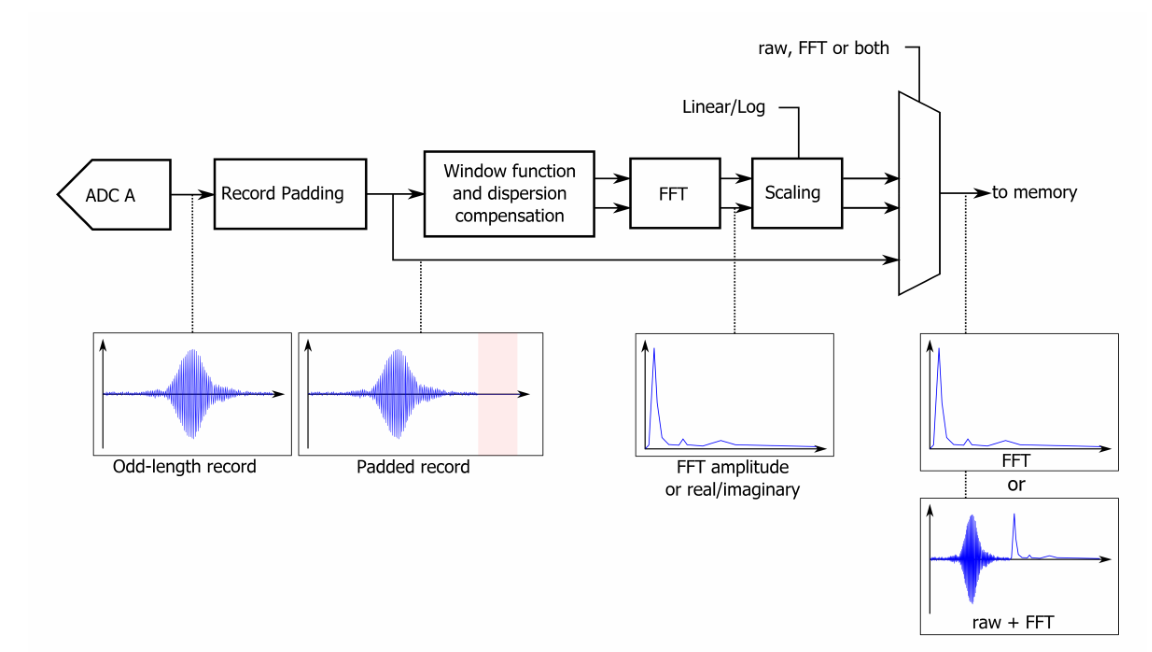
\includegraphics[width=.95\linewidth]{gfx/ch3/fft-module}}
    	\caption{Time diagram of a NPT AutoDMA acquisition.}\label{fig:fft-module}
    \end{figure}
    
    The format of frequency-domain data can be chosen between amplitude, real or imaginary part of the signal and can be converted in either single-precision floating point or unsigned integer. 
    
    \subsection{External clocking}
    As previously stated, the ATS9350 provides an SMA input for external clocking. This connector supports both sinusoidal and \ac{LVTTL} signals, sampling on each rising edge of the clock. The input impedence of the port is fixed at 50 $\Omega$ and AC coupling is used.
    
    There are three types of supported external clock operations:
    \begin{enumerate}
    	\item 10 MHz Reference Clock
    	\item Slow External Clock, 0 -- 60 MHz
    	\item Fast External Clock, 2 -- 500 MHz
    \end{enumerate} 

	Only the third mode is relevant for our application, as the $k$-clock provided by the Axsun SSOCT-1310 ranges from 180 to 340 MHz. A useful feature of the ATS9350 digitizer is the \emph{dummy clock switchover}: inbetween frequency sweeps some SS-OCT sources generate unstable clocks that do not respect the specification of the board; such behaviour could lead to missed trigger events. In order to avoid this issue, the board can switch to an internally generated clock for a specified amount of time after each record, and switch back to the external source once a trigger signal is detected. 
	
	
    \begin{figure}[bth]
    	\myfloatalign
    	{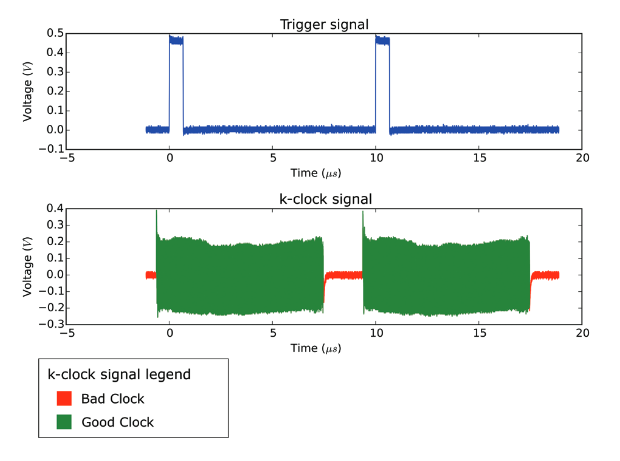
\includegraphics[width=.95\linewidth]{gfx/ch3/dummy-clock}}
    	\caption{Example of bad k-clock that requires the use of the dummy clock switchover.}\label{fig:dummy-clock}
    \end{figure}
    
    The use of this feature was not necessary in our case, as the installation of a k-clock deglitching firmware was enough to solve any problem related to bad clocks. 
    
    \subsection{Triggering}
    The acquisition of A and B-scans requires the ATS9350 to be configured in the following way:
    
    \begin{enumerate}
    	
    	\item The acquisition mode must be set to NPT AutoDMA.
    	
    	\item The laser sweep trigger, whose rising edge corresponds to the start of an A-scan, is connected to the External Trigger port of the board; as stated above, each record corresponds to an A-scan. The number of samples per A-scan should respect the following rules:\marginpar{The first two rules are needed for a correct alignment of the samples in memory.}
    	\begin{enumerate}
    		\item it should be a minimum of 256
    		\item it should be a multiple of 32
    		\item it should be less or equal to the number of sampling clocks of the $k$-clock, as specified by the manufacturer of the laser
    	\end{enumerate}
    
    	In our case the number of useful clocks per A-scan is 1536 (\autoref{tab:axsun-datasheet}), which also satisfies the first two rules. A conservative approach would require to set this number to $1536-32 =1504$, as a minor instability in the laser-generated clock could lead to a number of sampling clocks which is slightly lower, requiring the board to wait for the following A-scan to fill the record and consequently miss a trigger event. 
    	
    	The number of records per buffer instead determines the width of the B-scan. 
    	
    	\item  To start the acquisition of a B-scan, the Auxiliary port of the board must be configured as "Trigger Enable In" and a TTL pulse must be supplied to the connector. Once the board detects a rising edge on the AUX port, it will wait for a sufficient number of A-scan triggers to fill a buffer. Once the buffer has been filled a DMA transfer will be started and the image will be delivered to the user application.
    	Afterwards, the board waits for another pulse on the AUX port and start the acquisition of a new B-scan. 
    \end{enumerate}
    
    A more in-depth explanation of the programming of the board will be given in \autoref{ch:results}.
    
    
   
   
\newpage
\section{Optical Circuit}

In this section I will detail the process of designing and balancing the fiber optic interferometer that was used to realize the OCT device. Additionally, some performance parameters will be assessed. 


\subsection{Fiber Couplers}
In order to build a fiber optic interferometer, a device called \emph{fiber coupler} must be used. A coupler is a 4-port passive device which is typically used as a signal splitter/adder and that looks like the following:

\begin{center}
	{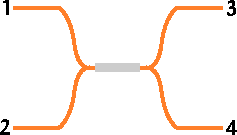
\includegraphics[width=0.35\linewidth]{gfx/ch3/couplers/fiber-coupler.pdf}}
\end{center}



The two couples of ports (1,2) and (3,4) are isolated, meaning that a signal that enters the device from port 1 (2) will not exit from port 2 (1) (the same principle holds for ports 3 and 4).  The "direct" paths ($1\xleftrightarrow{}3 $, $2\xleftrightarrow{} 4$) only let through a fraction of optical power equal to $|\rho|^2$ with no phase shift while the "crossed" paths ($1\xleftrightarrow{}4 $, $2\xleftrightarrow{} 3$) let through a fraction $1-|\rho|^2$ with a $\pi/2$ phase shift. The scattering matrix of this device is thus easily computed:

\begin{equation}
	S = \begin{bmatrix}
	0 & 0 & \rho & j\sqrt{1-\rho^2}\\
	0 & 0 & j\sqrt{1-\rho^2}& \rho \\
	\rho & j\sqrt{1-\rho^2}  & 0 & 0\\
	j\sqrt{1-\rho^2} & \rho  & 0 & 0
\end{bmatrix}
\end{equation}


For a 50:50 fiber coupler, $\rho = 1/\sqrt{2}$ so that 50\% of the optical power entering from e.g. port 1, will exit from port 3 and the other 50\% from port 4. 

For this thesis, three fiber couplers were used:
\begin{itemize}
	\item 2 Thorlabs TW1300R5A2\footnote{\url{https://www.thorlabs.com/thorproduct.cfm?partnumber=TW1300R5A2}} 50:50 fiber couplers
	\item 1 Thorlabs TW1300R2A2\footnote{\url{https://www.thorlabs.com/thorproduct.cfm?partnumber=TW1300R2A2}} 90:10 fiber coupler	
\end{itemize} 
The arms of the couplers are color coded to easily distinguish the direct paths, which are White$\xleftrightarrow{}$White and Blue$\xleftrightarrow{}$Red.

\subsection{Measuring the couplers' length}
For the design of the interferometer it is useful to determine the length of the coupler's arms with high precision. This was accomplished using an \acf{OFDR} and the setup in \autoref{fig:setup-couplers-length}. 


\begin{figure}[bth]
	\myfloatalign
	{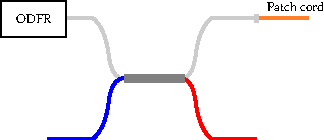
\includegraphics[width=0.5\linewidth]{gfx/ch3/couplers/setup-misura-lunghezza.pdf}}
	\caption{Diagram of setup for the measurement of fiber couplers' length.}\label{fig:setup-couplers-length}
\end{figure}


For each input put, the \ac{OFDR} trace will contain two peaks corresponding to the reflections generated by the fiber/air interface of the two non-isolated ports, which can be used to determine the length of the optical paths. In order to associate a spefic port to its peak, a fiber patch cord was connected to the port, resulting in the reduction of the corresponding peak in the trace. For the same input port a second trace is acquired, switching the position of the patch cord. This procedure is repeated for each of the 4 input ports, for a total of $8$ traces per coupler. 

The resulting traces are available in \autoref{ch:appendixA}. The total length of each path and the difference in length between adjacent arms are summarized in \autoref{tab:couplers-length} and \autoref{tab:couplers-diff} respectively.



\begin{table}
	\begin{tabularx}{\textwidth}{Xlll} \toprule
		& \multicolumn{3}{c}{Path length [mm]}\\
		\tableheadline{Path} & \tableheadline{50-50A} & \tableheadline{50-50B} & \tableheadline{90-10}
		\\ \midrule
		White $\xleftrightarrow{}$ White &  2101.9939   & 2098.610325 &  2112.5832\\
		White $\xleftrightarrow{}$ Red   &  2108.25695  & 2119.471656 &  2113.8573\\
		White $\xleftrightarrow{}$ Blue  &  2101.149125 & 2095.978125 &  2129.024925\\
		Blue $\xleftrightarrow{}$ Red    &  2107.402875 & 2116.86915  &  2130.299\\
		\bottomrule
	\end{tabularx}
	\caption{Length of the paths of the fiber couplers.}\label{tab:couplers-length}
\end{table}

\begin{table}
	\begin{tabularx}{\textwidth}{Xlll} \toprule
		& \multicolumn{3}{c}{Path length difference [mm]}\\
		\tableheadline{Arms couple} & \tableheadline{50-50A} & \tableheadline{50-50B} & \tableheadline{90-10}
		\\ \midrule
		White-Blue  &  0.84   & 2.62 &  16.44\\
		White-Red   &  6.25   & 20.85 &  1.28\\
		\bottomrule
	\end{tabularx}
	\caption{Path difference of each pair of adjacent ports of the couplers.}\label{tab:couplers-diff}
\end{table}



\subsection{ Mach-Zender Interferometer }
In order to test the \ac{DAQ} device and to determine the effect of sampling an interference signal with laser-supplied $k$-clock, a simple unbalanced \ac{MZI} was set up using two 50-50 fiber couplers. The diagram of the setup for this test is reported in \autoref{fig:unbalanced-mzi}. In order to acquire a beat frequency with the ATS9350, two replicas of the laser pulse have to overlap with a relative delay $\tau$ that is less than the source coherence time. Additionally, the beat frequency has to fall in the electronic bandwidth of 1) the photodiodes and 2) the acquisition device. The delay element in the unbalanced interferometer arises from the difference in length of the couplers' arms. 


\begin{figure}[bth]
	\myfloatalign
	{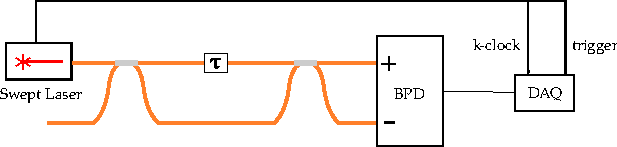
\includegraphics[width=\linewidth]{gfx/setup-diagrams/interferometer.pdf}}
	\caption{Diagram of an unbalanced Mach-Zender Interferometer.}\label{fig:unbalanced-mzi}
\end{figure}


The swept laser emits a signal with a time-varying frequency that can be described as follows
\begin{equation}
E_{ss} = E_{in} e^{j2\pi f(t) t} = E_{in}e^{j\phi(t)},
\end{equation}
hence the signals at the input ports of the second coupler will be respectively
\begin{equation}
	E_1 = \frac{1}{\sqrt{2}}E_{in} e^{j\phi(t-\tau)}\quad
	E_2 = j\frac{1}{\sqrt{2}}E_{in} e^{j\phi(t)}
\end{equation}
The $+$ and $-$ ports of the BPD will instead see two signals expressed by
\begin{align}
	&E_+ = \frac{1}{2}E_{in} e^{j\phi(t-\tau)} - \frac{1}{2}E_{in} e^{j\phi(t)}\\
	&E_- = j\frac{1}{2}E_{in} e^{j\phi(t)} + j \frac{1}{2}E_{in} e^{j\phi(t-\tau)}
\end{align}
which will be converted by the photodiode in the following currents
\begin{align}
	& I_+ \propto \langle E_+ E_+^* \rangle = \frac{1}{2}|E_{in}|^2 - \frac{1}{2}\cos\left[\phi(t)-\phi(t-\tau)\right]\\
	& I_- \propto \langle E_- E_-^* \rangle = \frac{1}{2}|E_{in}|^2 + \frac{1}{2}\cos\left[\phi(t)-\phi(t-\tau)\right]
\end{align}
The output of the BPD will then be the sum the two currents
\begin{equation}
	I_{tot} = I_+ - I_- \propto \cos\left[\phi(t)-\phi(t-\tau)\right].
\end{equation}
We can observe that the DC term has been canceled out, leaving only an oscillating term that depends on the phase of the light source. 


If the frequency sweep of the laser is assumed linear, the \ac{BPD} generates a sinusoidal current with frequency that is proportional to the \ac{OPD} between the arms of the interferometer:
\begin{equation}
	I_{tot} \propto \cos \left[ 2\pi \sigma_f\tau t +\phi_0 \right].
\end{equation}
The beat frequency is determined by the \ac{OPD} $\Delta z$ through the following relation
\begin{equation}\label{eq:mzi-freqtoopd}
	f = \sigma_f \tau = \sigma_f \frac{n\Delta z}{c_0},
\end{equation}
where $n=1.4674$ is the refractive index of the optical fiber used for the manufacturing of the couplers\footnote{\url{https://www.corning.com/media/worldwide/coc/documents/PI1463_07-14_English.pdf}} and $c_0$ is the speed of light in vacuum. 

Connecting the White and Red ports of coupler A to the White and Blue ports of coupler B we obtain $\Delta z = 6.25-2.62\approx 3.63$ mm (\autoref{tab:couplers-diff}), which corresponds to a beat frequency $f \approx 87$ MHz. This frequency is sufficiently low to satisfy Nyquist's criterion and be sampled using the $k$-clock, as its maximum frequency is $\approx 330$ MHz. 

The total BPD current was acquired with the ATS9350 digitizer using the provided AlazarDSO software. Two acquisitions were made, first using the internal 500 MHz clock and then clocking the board with the $k$-clock. In order to synchronize the acquisition with the laser sweep, the board was externally triggered by the sweep-start signal supplied by the laser. 

When acquiring with the internal clock, the number of useful samples to acquire was calculated as follows
\begin{equation}
	N = F_s \frac{d_c}{f} = 2525,
\end{equation}
where $F_s=500$ MHz is the sampling frequency, $d_c = 0.505$ is the laser duty cycle and $f=100$ kHz is the sweep repetition rate. In order to satisfy the bit alignment requirement of the board, the actual number of samples was set to the nearest multiple of 32, $\hat{N}=2528$. Instead, when using the external clock option of the board, this number is determined by the number of useful sampling instants of the $k$-clock, $1536$ (\autoref{tab:axsun-datasheet}).  

The acquired signals were multiplied by a Hamming window and then Fourier-trasformed. The result of this procedure is illustrated in \autoref{fig:mzi-comparison}, where the x-axis is mapped from frequency to OPD by inverting \autoref{eq:mzi-freqtoopd}. We can notice that when using the internal clock of the board, the frequency content of the signal is spread over a relatively wide band (left). In fact, since the frequency sweep is not linear, uniformly sampling the interference signal results in a distorted sinusoidal term. Thus,  a precise estimation of the OPD between the \ac{MZI} arms is not possible. 


\begin{figure}[hbt]
	{\myfloatalign
		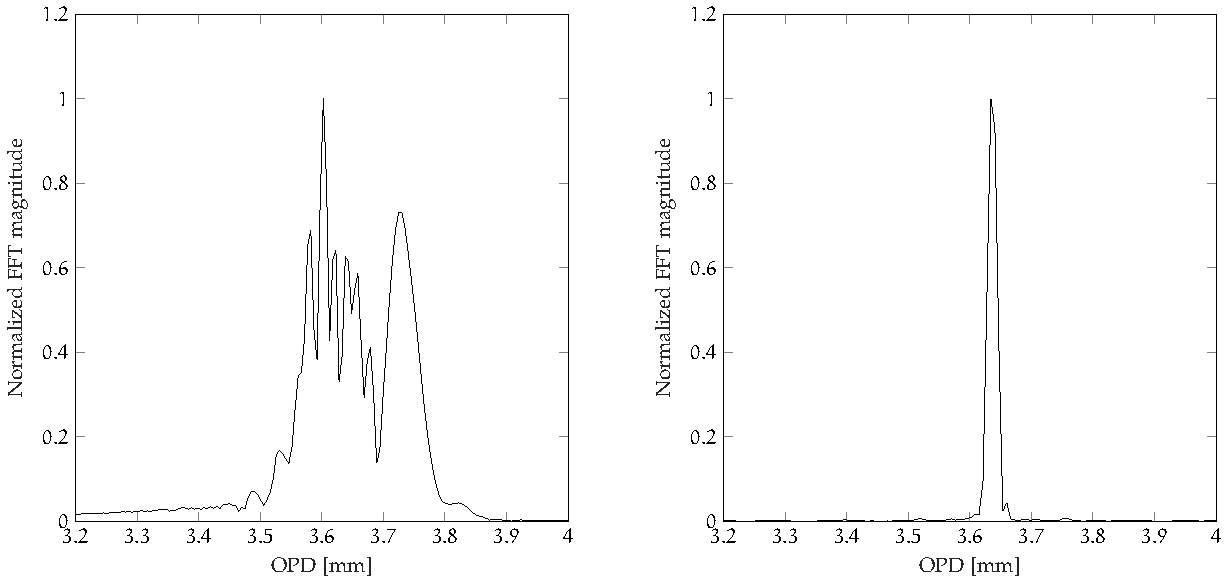
\includegraphics[width=\linewidth]{gfx/ch3/interferometer/interferometer}}
	\caption{Comparison between the beat frequency acquired with the uniform clock (left) and the $k$-clock (right).}\label{fig:mzi-comparison}
\end{figure}

On the other hand, sampling with the provided $k$-clock produces a clearly defined peak in the frequency domain (right) and permits a precise evalutation of the OPD. 

To better appreciate the effect of external clocking on the imaging quality of an OCT system, a number of $W = 1000$ consecutive A-scans were captured, from which an artificial B-scan was generated (\autoref{fig:mzi-frame}). 


\begin{figure}[hbt]
	{\myfloatalign
		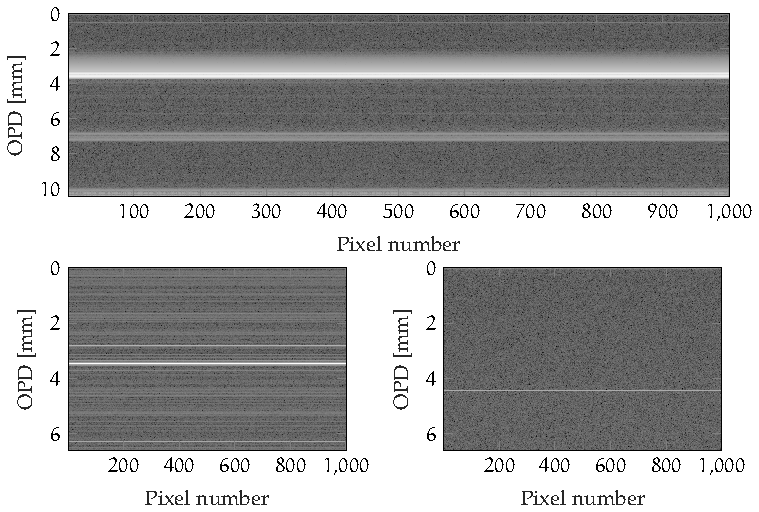
\includegraphics[width=\linewidth]{gfx/ch3/interferometer/interferometer-frame}}
	\caption{Simulated B-scans using the internal 500 MHz clock (top) and the $k$-clock (bottom).}\label{fig:mzi-frame}
\end{figure}

Using the internal clock and a logarithmic color scale (top), the width of the peak is significantly more pronounced: in this case a perfect reflector would take up a considerable portion of the imaging range. Moreover, the axial resolution of the OCT would not be acceptable for a functioning system. In this image it is also possible to notice two faint peaks at $\sim 7$ mm and $\sim 10$ mm. These are due to reflections accumulating a delay which is a multiple of the OPD between the arms of the interferometer. 

As expected, the improvement when sampling with the $k$-clock is remarkable (bottom left). We can also notice that since the frequency of the $k$-clock is smaller than 500 MHz, the second of the two peaks generated by reflections is undersampled and appears at $\sim 2.5$ mm. The third image (bottom right) was captured after distancing the APC connectors on one of the arms of the \ac{MZI}, introducing a $\sim 1$ mm layer of air ($n=1$) which corresponds to an additional $\sim 0.68$ mm of OPD in the fiber. The reflection peaks in this case do not appear as the received power is too low. 


\subsection{Fiber Michelson interferometer}

The first OCT circuit that was tested was a simple Michelson interferometer realized with a 50-50 fiber coupler. The schematic diagram of this setup is illustrated in \autoref{fig:basic-oct}. The reference arm consists in a cage system with a silver mirror mounted on a translatable support and an adjustable FiberPort collimator (\autoref{fig:reference-arm-photo}). This collimator permits a fine aligment with five degrees of freedom to easily maximize the amount of power that gets coupled back in the optical fiber after being reflected by the mirror. Through a careful alignment procedure, the attenuation of the reference arm is minimized, reaching a value of $\sim 4$ dB. 


\begin{figure}[bth]
	\myfloatalign
	{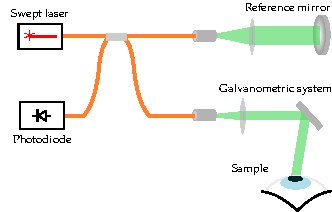
\includegraphics[width=0.8\linewidth]{gfx/setup-diagrams/basic-oct.pdf}}
	\caption{SS-OCT setup using a fiber Michelson interferometer.}\label{fig:basic-oct}
\end{figure}


\begin{figure}[bth]
	\myfloatalign
	{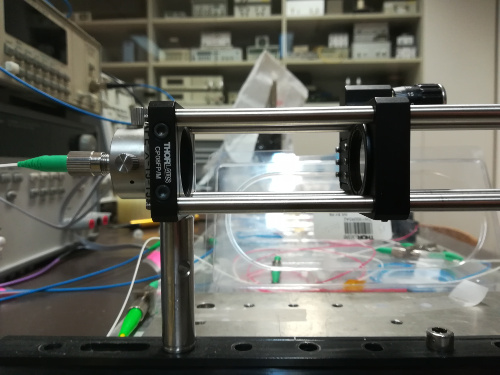
\includegraphics[width=0.6\linewidth]{gfx/ch3/reference-arm-photo}}
	\caption{SS-OCT setup using a fiber Michelson interferometer.}\label{fig:reference-arm-photo}
\end{figure}

This setup, while fairly simple, gave rise to two different issues:
\begin{enumerate}
	\item a balanced detection scheme could not be implemented.
	
	\item the output of the optical source experienced instability, as half of the power reflected by the two arms is coupled back in the laser output port. This behaviour was tested by replacing the reference arm with a photodiode and monitoring its current. In \autoref{fig:first-scheme-instability} we can see that the power profile of the source is substantially distorted when a high-reflectivity object such as a mirror is placed under the focusing lens of the sample arm. With the additional power reflected by the reference mirror this behaviour can only worsen. 
	
	
\end{enumerate}
\begin{figure}[bth]
	\myfloatalign
	{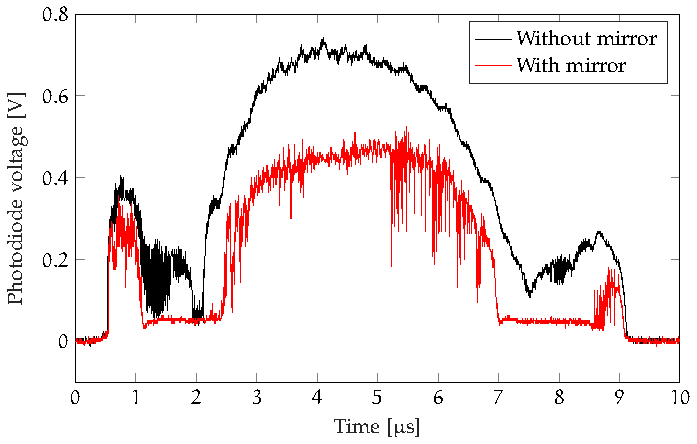
\includegraphics[width=0.8\linewidth]{gfx/ch3/first-scheme-instability}}
	\caption{Instability of the laser output power.}\label{fig:first-scheme-instability}
\end{figure}




\subsection{Second scheme}
In order to limit the amount of power returning to the laser and avoid permanent damage, the setup in \autoref{fig:final-setup} has been designed. Connecting the source to the 90-10 coupler, only 10\% of the total output power is directed to the sample and only 10\% of the reflected power is directed back to the laser, reducing the reflected power by a factor of 25. The power profile of the source was measured by connecting a photodiode to connector D and monitoring its current. Unlike before, placing a mirror in the sample arm did not alter the shape of the laser pulse. 

With respect to the previous scheme, the power returning to the laser from the reference arm is attenuated by $\sim 2$ dB thanks to the 90-10 coupler. 
The effect of the reference arm on the stability of the laser output was tested in a similar way, connecting the photodiode to connector I. With the silver mirror stilll on the sample arm, the FiberPort collimator was slightly mis-aligned until the measured power profile did not exhibit any distortion. 

\begin{figure}[bth]
	\myfloatalign
	{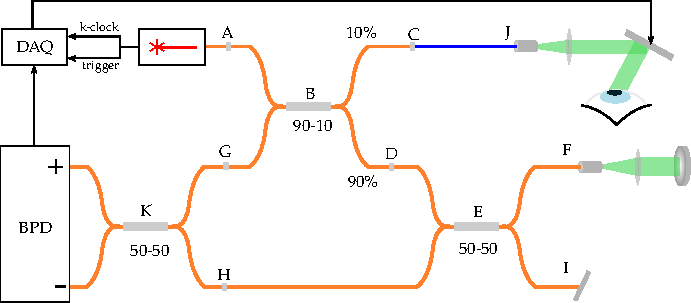
\includegraphics[width=\linewidth]{gfx/setup-diagrams/final-setup-2.pdf}}
	\caption{Final SS-OCT setup.}\label{fig:final-setup}
\end{figure}

\subsubsection{Balancing the interferometer}
As already explained, interference fringes are only visible if the mismatch between the length of sample and reference arm is less than the coherence length of the source.

With reference to \autoref{fig:final-setup}, the length of the sample arm, defined by the letters ABCJCBGK is
\begin{equation}
L_{\text{sample}} = \overline{\text{ABCJCBGK}} = 5L_{\text{arm}} + 2L_{\text{patch}},
\end{equation}
where $L_{\text{arm}}$ is the length of the couplers' arm and $L_{\text{patch}}$ is the length of the fiber patch cord (illustrated in blue). The reference arm is instead defined by the path ABDEFEHK, whose length is
\begin{equation}
	L_{\text{ref}} = \overline{\text{ABDEFEHK}} = 7L_{\text{arm}},
\end{equation}
meaning that, ideally
\begin{equation}
	| L_{\text{ref}} - L_{\text{sample}}| = 0 \implies L_{\text{patch}} = L_{\text{arm}},
\end{equation}
Since $L_{\text{arm}} \sim 1$ m, a patch cord of the same length has to be used. Potentially, light travelling the path ABDEFEDBGK could cause unwanted interference, but since
\begin{equation}
| L_{\text{ref}} - \overline{\text{ABDEFEDBGK}}| = 2L_{\text{arm}} \approx 2 \text{ m},
\end{equation}
the mismatch is far greater than the coherence length of the source, $l_c \approx 12$ mm meaning that no interference will be generated. 

This setup is therefore able to protect the laser source from damage caused by strong reflections, removes unwanted coherent noise and enables balanced detection. In order to minimize distortions due to the detection scheme, the BPD is connected to the fiber coupler with the smallest mismatch between adjacent ports: looking at \autoref{tab:couplers-diff}, the Blue and White arms of coupler 50-50 A are the optimal choice. 

\subsubsection{OFDR measurement}

For a more precise analysis on the balancing of sample and reference arm, the difference between the two optical paths is measured with an OFDR using the setup in \autoref{fig:obr-balancing-setup}. The optical circulator enables us to select the path to measure, obtaining traces that are easier to interpret, while the fiber attenuator is used as a safety measure to protect the OFDR receiver. 

\begin{figure}[hbt]
	\myfloatalign
	{	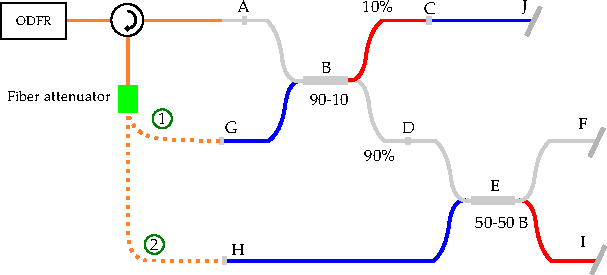
\includegraphics[width=\linewidth]{gfx/ch3/obr-balancing-setup}}
	\caption{Time signal when the optical path difference is close to 0.}\label{fig:obr-balancing-setup}
\end{figure}

The acquired traces are illustrated in \autoref{fig:obr-balancing}. From left to right we can observe:
\begin{itemize}
	\item The reflection coming from connector I, measured with the circulator connected to port 1. This is the "unwanted" reflection that was previously discussed. 
	
	\item The reflection coming from connector C, when no patch cord is connected.
	\item The reflection coming from connector J, corresponding to the end of the fiber patch cord. 
	
	\item The two reflections coming from connectors F and I. As we can see, the two are distanced by $\sim 2$ centimeters, confirming the measurements reported in \autoref{tab:couplers-diff}. 
\end{itemize}

Connecting the reference system to connector F, the path length difference becomes $\Delta L \approx 35$ mm. Since the interference between the two signals occurs in the fused part of coupler 50-50 A (point K in \autoref{fig:final-setup}), the length mismatch of its White and Red arms ($\approx 6.2$ mm) can be exploited to bring the total \ac{OPD} down to $\Delta L \approx 29$ mm. These 3 centimeters can be compensated with the translatable mirror in the reference arm. 




\begin{figure}[hbt]
	\myfloatalign
	{	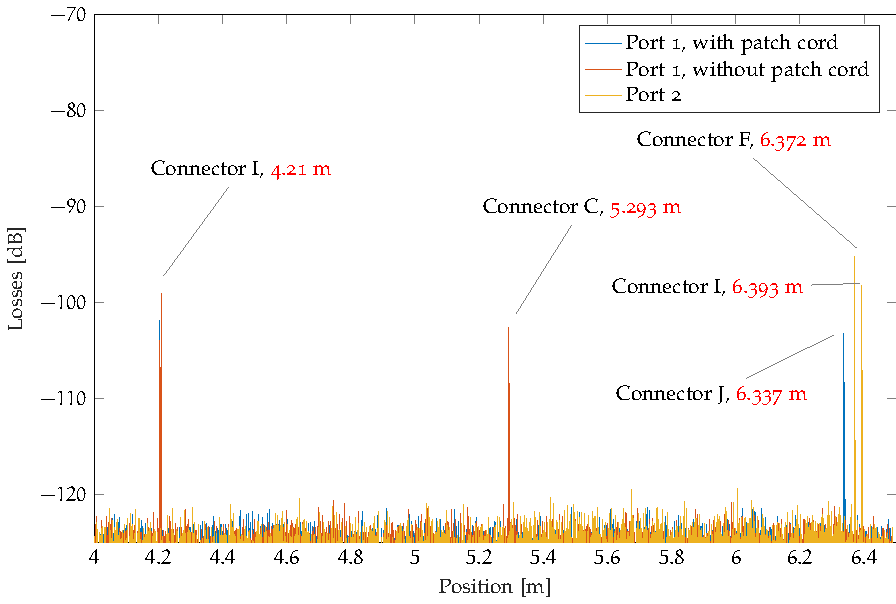
\includegraphics[width=\linewidth]{gfx/ch3/obr-balancing}}
	\caption{OFDR traces used to balance the interferometer.}\label{fig:obr-balancing}
\end{figure}



\begin{figure}[hbt]
	\myfloatalign
	{	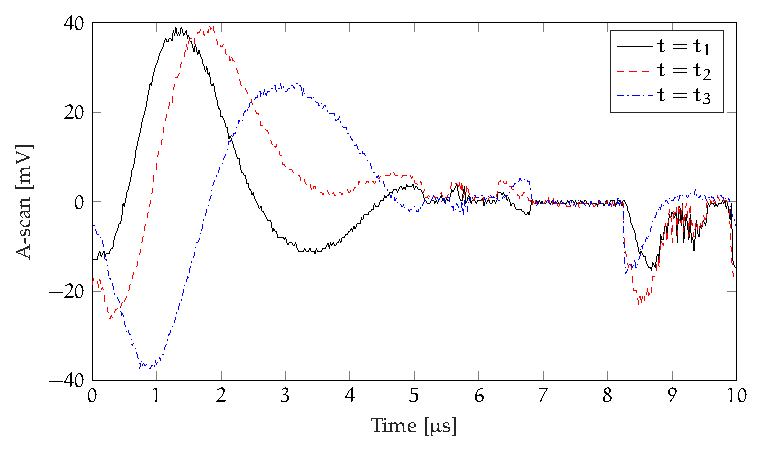
\includegraphics[width=\linewidth]{gfx/tikz/balancing/balanced}}
	\caption{Time signal when the optical path difference is close to 0.}\label{fig:signal-balanced}
\end{figure}

\begin{figure}[hbt]
	\myfloatalign
	{	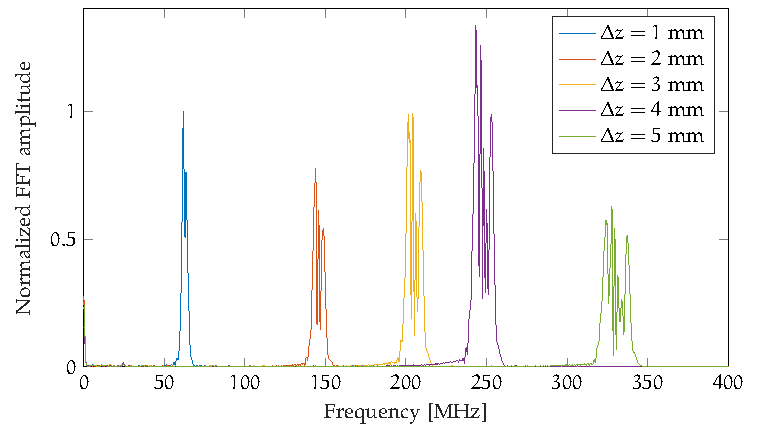
\includegraphics[width=\linewidth]{gfx/tikz/balancing/unbalanced}}
	\caption{Effect of reference arm unbalancing on the beat frequenc
		y}\label{fig:unbalanced-spectrum}
\end{figure}


\subsection{Signal-to-noise ratio profile}

Try with new measurements

\subsection{Thickness measurements}
No scattering detected, only reflections caused by the surface


\begin{figure}[hbt]
\myfloatalign
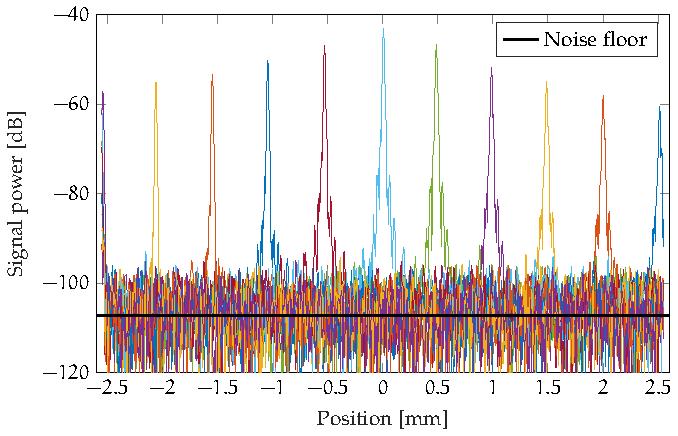
\includegraphics[width=\linewidth]{gfx/falloff}
\caption{Signal spectrum at various depths.}\label{fig:power-falloff}
\end{figure}


\begin{figure}[hbt]
\myfloatalign
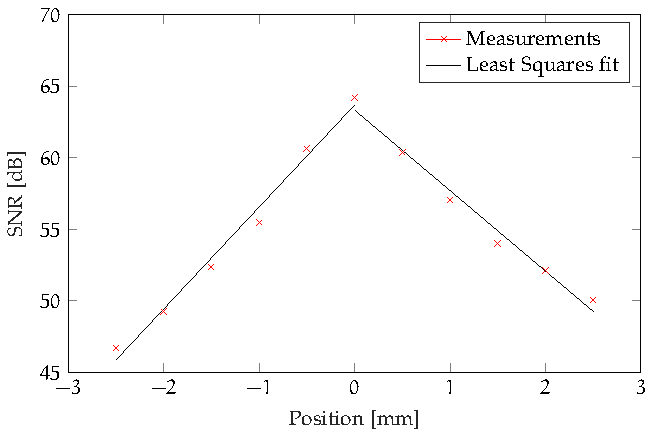
\includegraphics[width=0.9\linewidth]{gfx/falloff-fit}
\caption{Signal-to-noise ratio falloff.}\label{fig:falloff-fit}
\end{figure}



\begin{figure}[hbt]
\centering
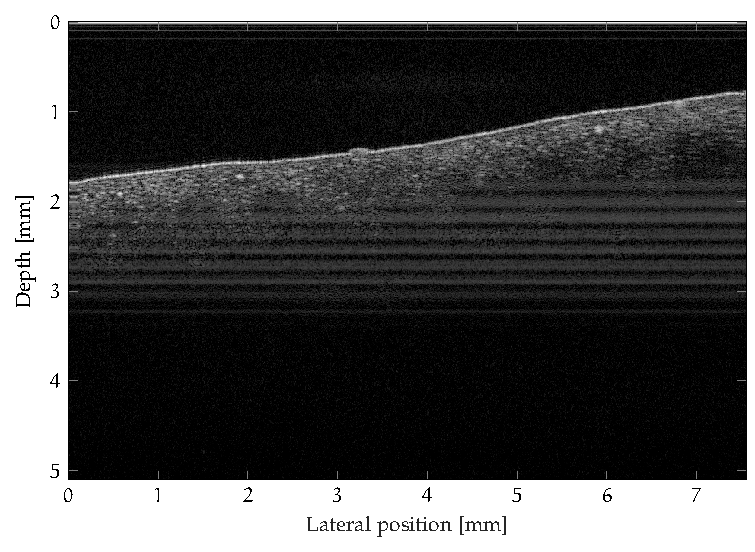
\includegraphics[width=\linewidth]{gfx/tikz/axsun/banana-peel}
\caption{B-scan of banana peel.}\label{fig:banana-peel}
\end{figure}%----------------------------------------------------------------------------------------
\begin{figure}[hbt]
\myfloatalign
{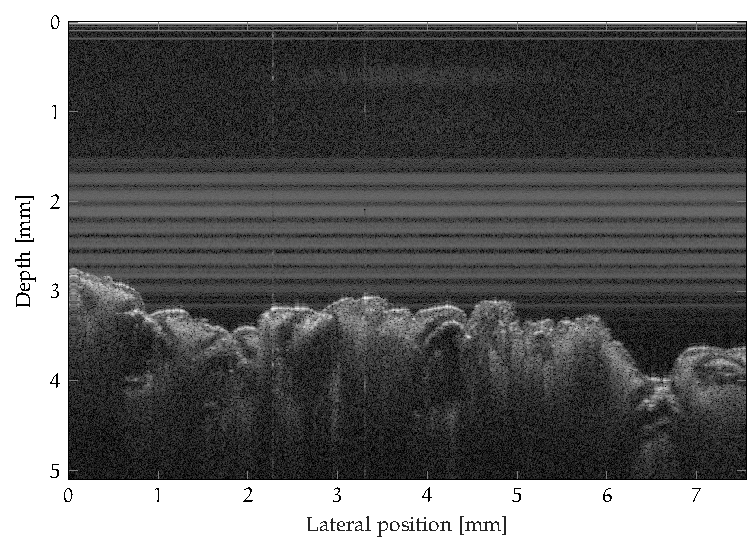
\includegraphics[width=\linewidth]{gfx/tikz/axsun/dry-orange-peel}}
\caption{B-scan of dry orange peel.}\label{fig:dry-orange-peel}
\end{figure}%----------------------------------------------------------------------------------------

\begin{figure}[hbt]
\myfloatalign
{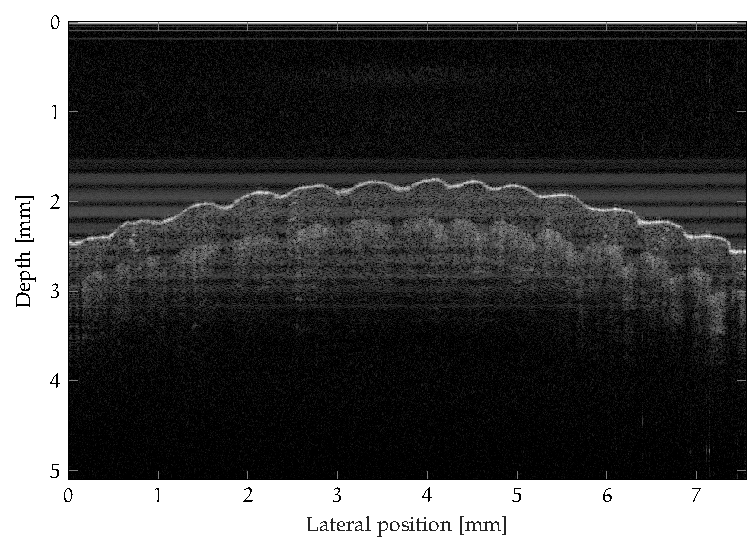
\includegraphics[width=\linewidth]{gfx/tikz/axsun/finger}}
\caption{B-scan of a human finger.}\label{fig:finger}
\end{figure}%----------------------------------------------------------------------------------------
%----------------------------------------------------------------------------------------
